\documentclass{beamer}
%
% Choose how your presentation looks.
%
% For more themes, color themes and font themes, see:
% http://deic.uab.es/~iblanes/beamer_gallery/index_by_theme.html
%
\mode<presentation>
{
  \usetheme{default}      % or try Darmstadt, Madrid, Warsaw, ...
  \usecolortheme{default} % or try albatross, beaver, crane, ...
  \usefonttheme{default}  % or try serif, structurebold, ...
  \setbeamertemplate{navigation symbols}{}
  \setbeamertemplate{caption}[numbered]
} 

\usepackage[czech, russian]{babel}
\usepackage[utf8]{inputenc}
\usepackage{xcolor}
\usepackage{ulem}
\usepackage{pdfpages}
\usepackage{listings}
\usepackage{verbatim}
\usepackage{skak}
\usepackage{chessboard}
\usepackage[table]{xcolor}
\def\mainlinestyle{\bfseries}
\def\variationstyle{}
\usepackage{tikz}
\usetikzlibrary{arrows.meta}


 


\title[HKUI]{HKUI - \LaTeX}
\author{Pavel Jedli\v{c}ka}
\institute{Západočeská univerzita v Plzni}
\date{\today}

\begin{document}
\selectlanguage{czech}

\begin{frame}
  \titlepage
  
\end{frame}

% Uncomment these lines for an automatically generated outline.
%\begin{frame}{Outline}
%  \tableofcontents
%\end{frame}

\section{úvod}
\begin{frame}{Latex? Co je to?}
\centering
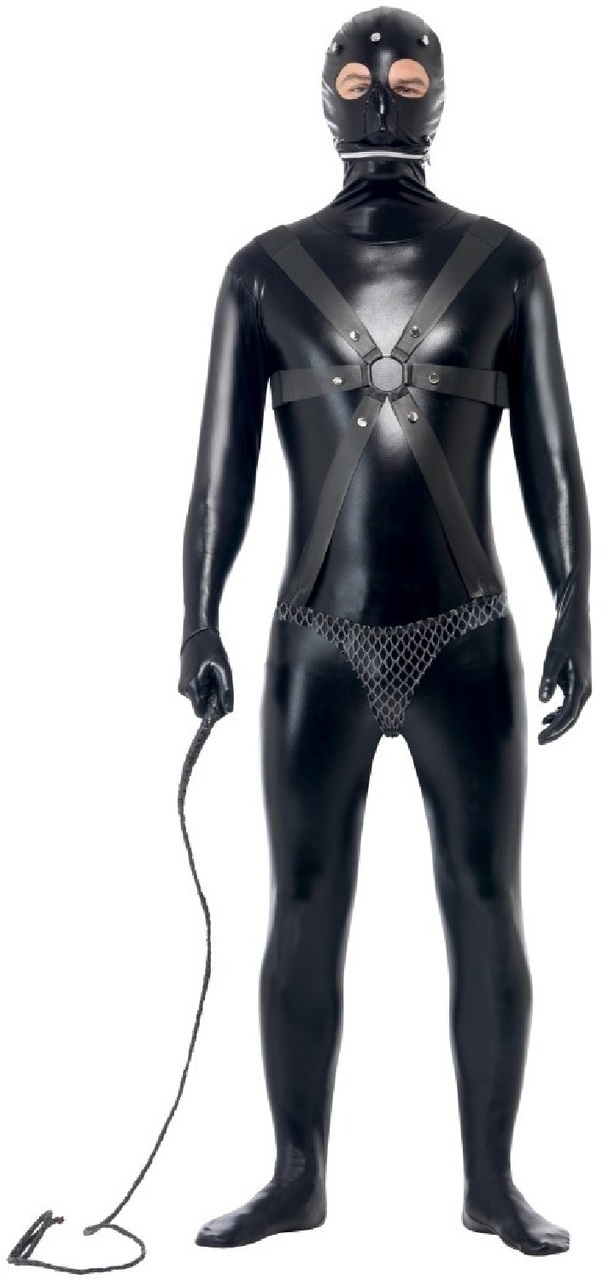
\includegraphics[width=.3\textwidth]{pic/latex_fun.jpg}
\caption{Tohle je latex. \footnote{Zdroj: Smiffy's Men's Gimp Costume Bodysuit with Straps and Chainmail Pants @ Amazon (from $\$$ 26.49)}}
\end{frame}


\begin{frame}{\LaTeX? Co je to?}
\begin{itemize}
    \item \TeX: program pro sazbu textu. 
    \vspace{1cm}
    \item \LaTeX: sada maker pro \TeX, usnadňující práci (nejen) pro uživatele bez znalostí sazby. 
\end{itemize}
\end{frame}


\begin{frame}{Proč používat \LaTeX}
\begin{figure}
      \centering
      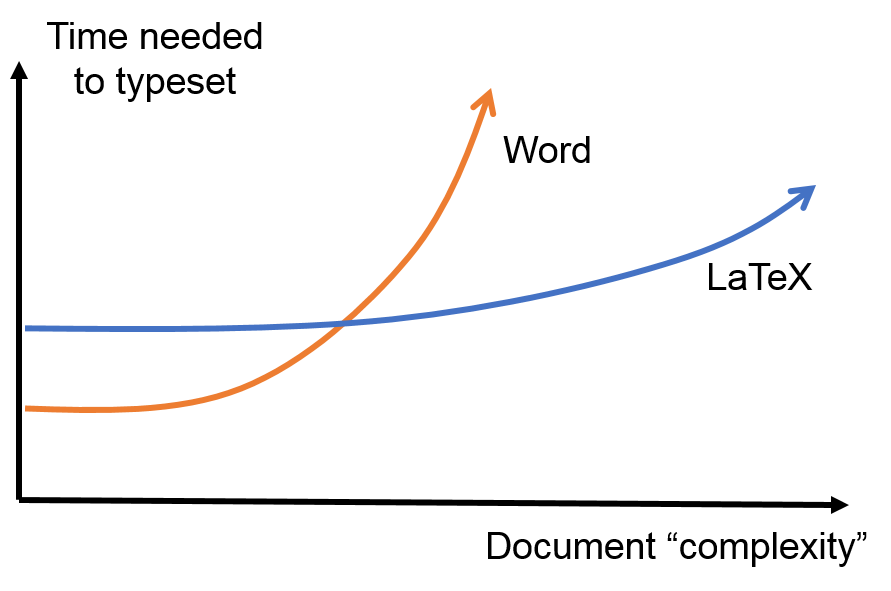
\includegraphics[width=.7\textwidth]{pic/word_vs_latex_1_eng.png}
      \caption{\LaTeX vs Word.\footnote{Zdroj: J. L. Blanco, mappingignorance.org} }
      \label{fig:my_label}
  \end{figure}{}
\end{frame}


\section{ukázka}
\begin{frame}{Jak to vypadá?}
word:
\frame{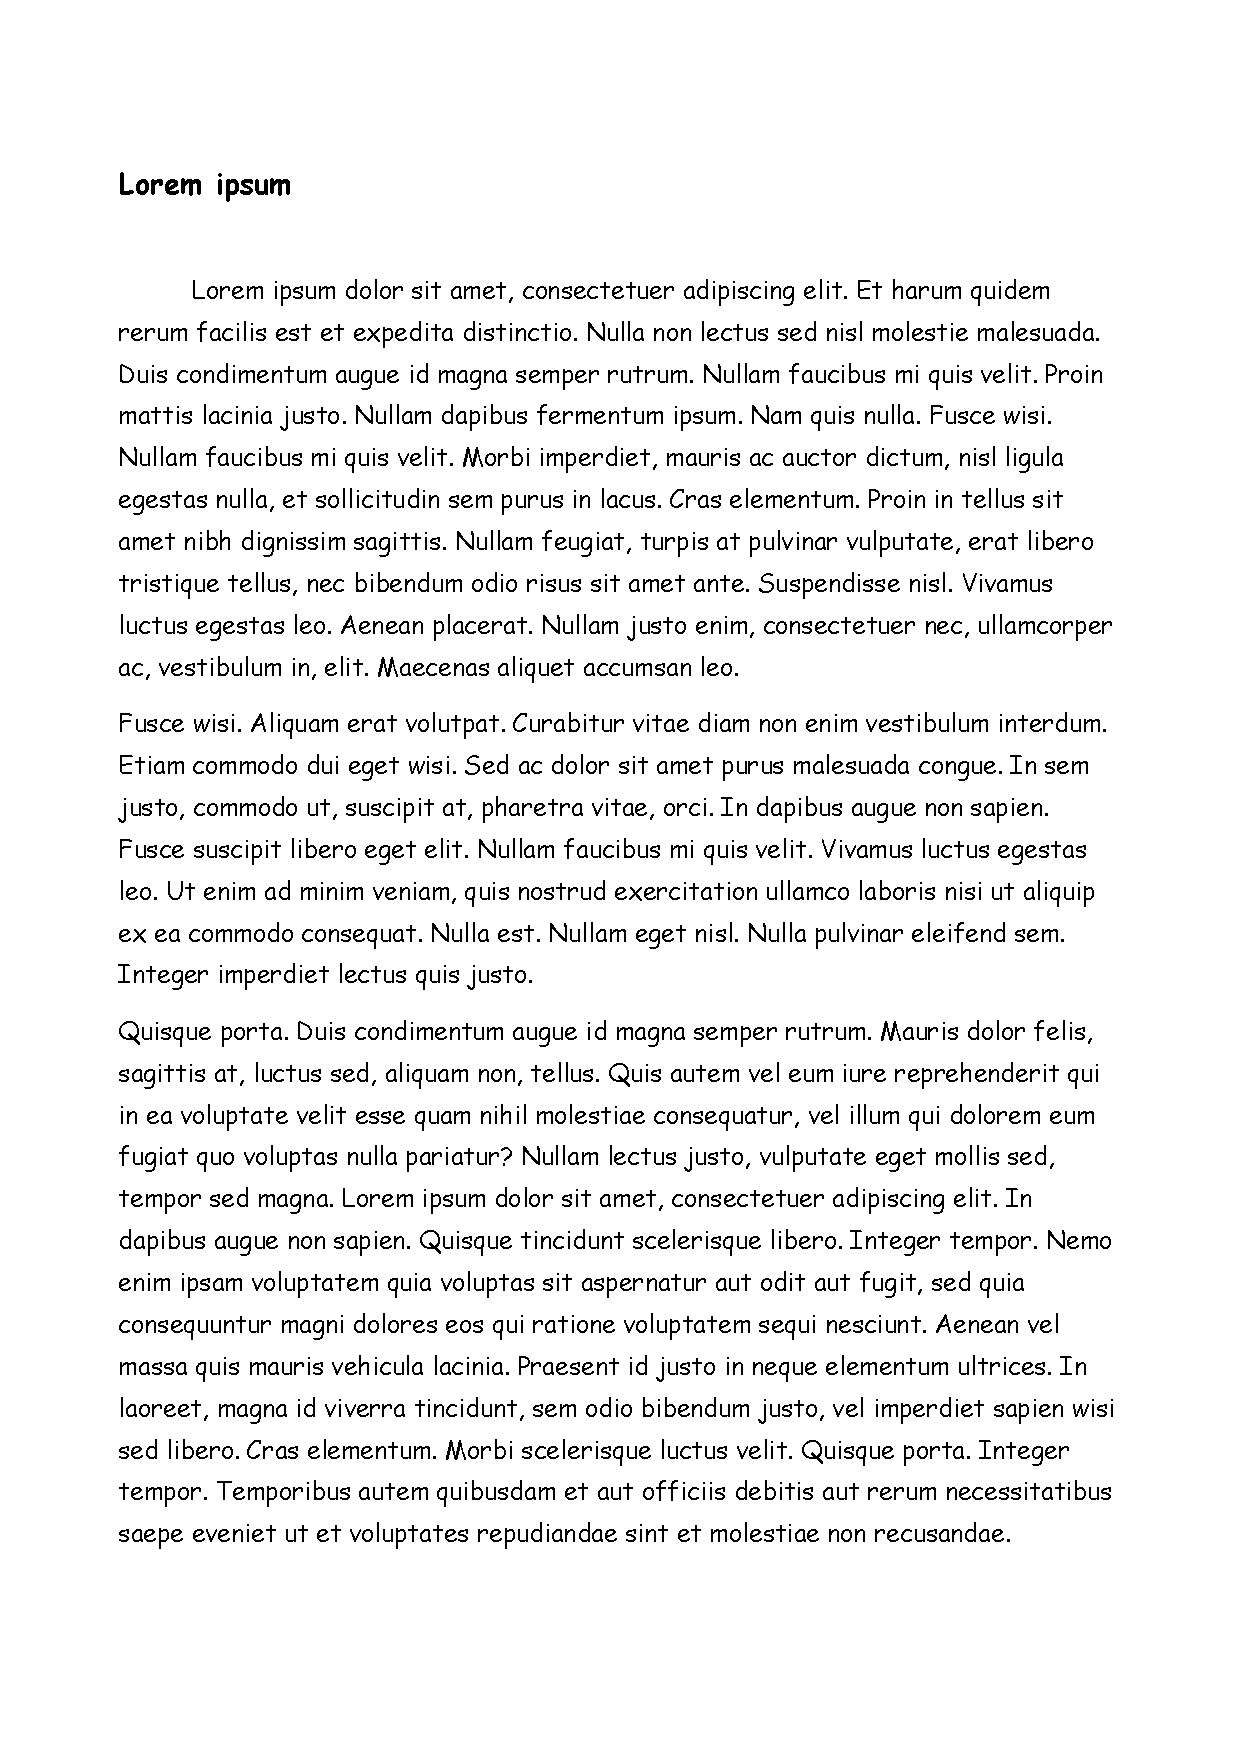
\includegraphics[width=\textwidth]{word_lorem.pdf}}
\end{frame}{}

\begin{frame}{Jak to vypadá?}
latex:
\frame{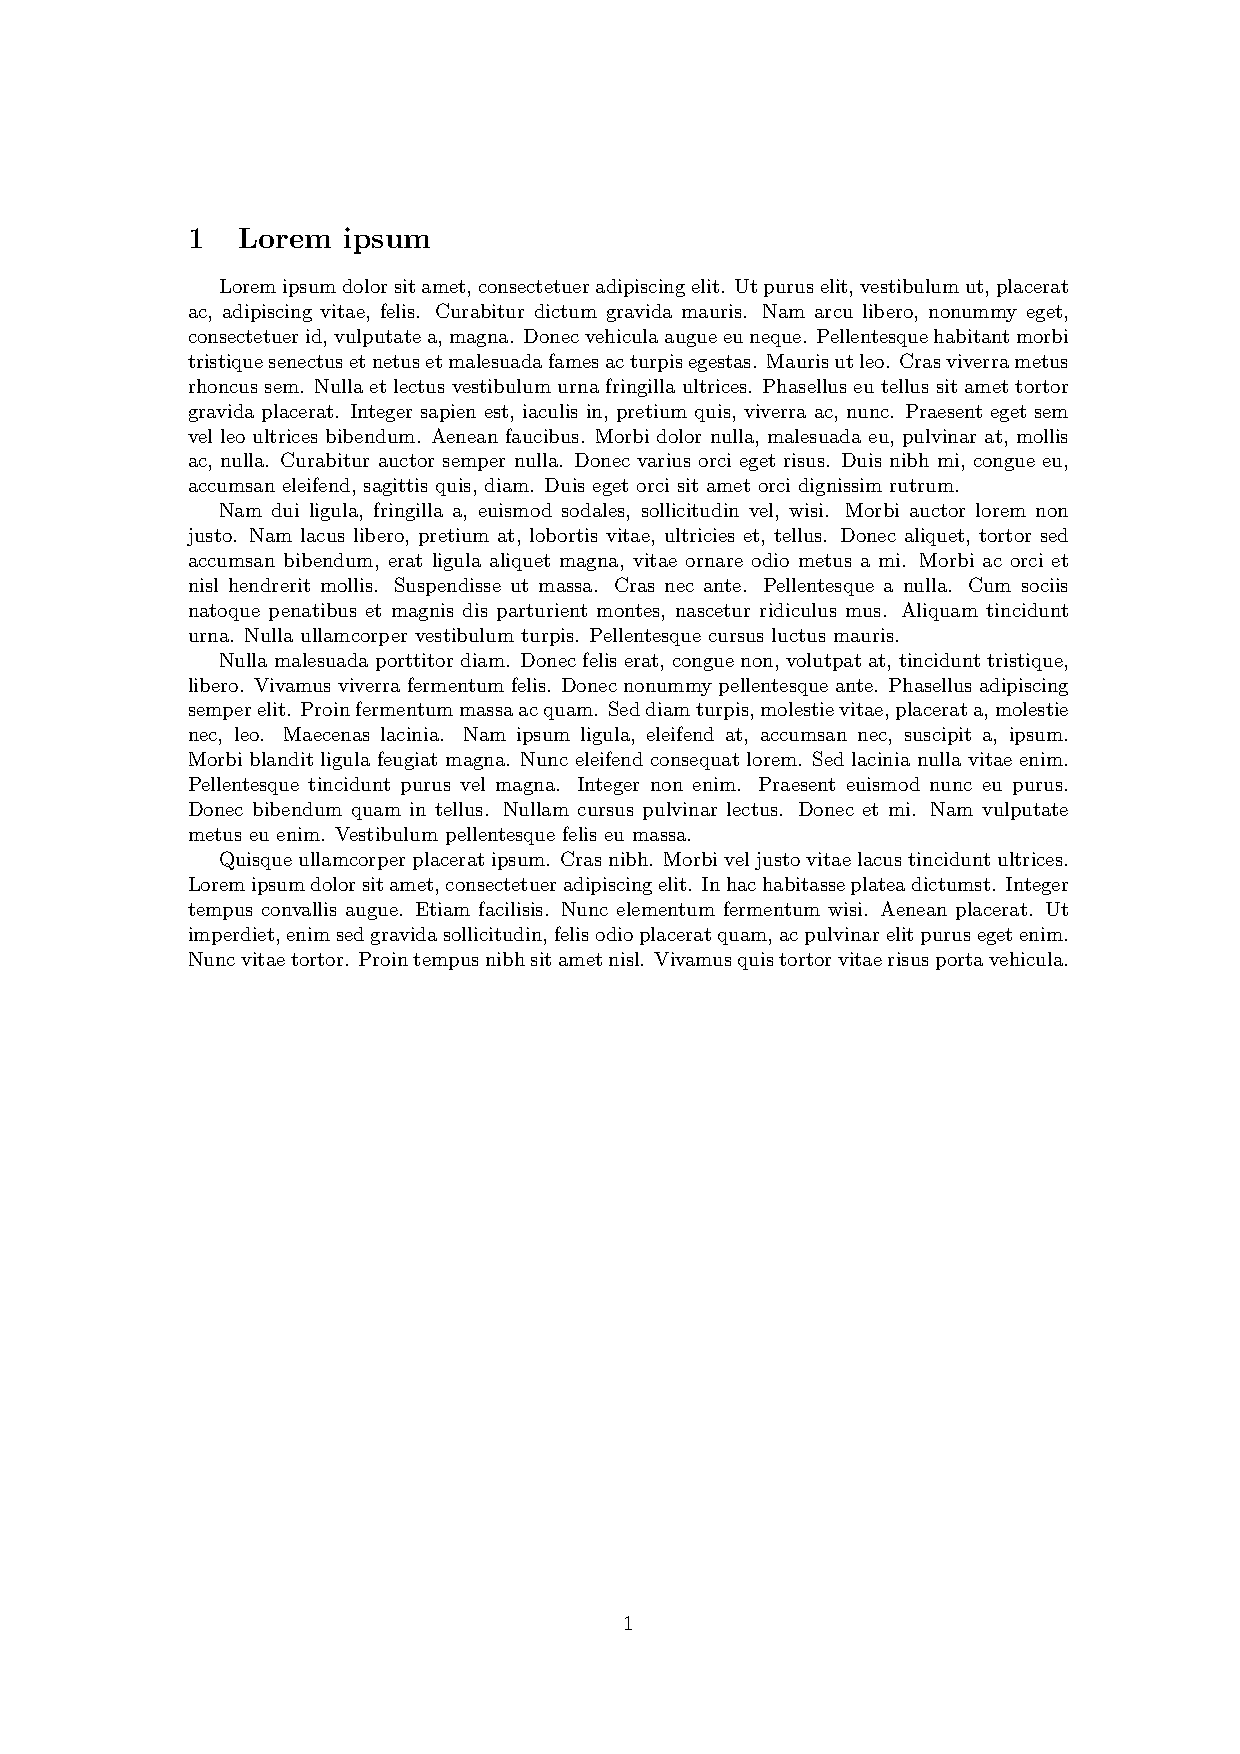
\includegraphics[width=\textwidth]{lipsum.pdf}}
\end{frame}{}

\section{příklad}
\begin{frame}{Jak se v tom píše?}
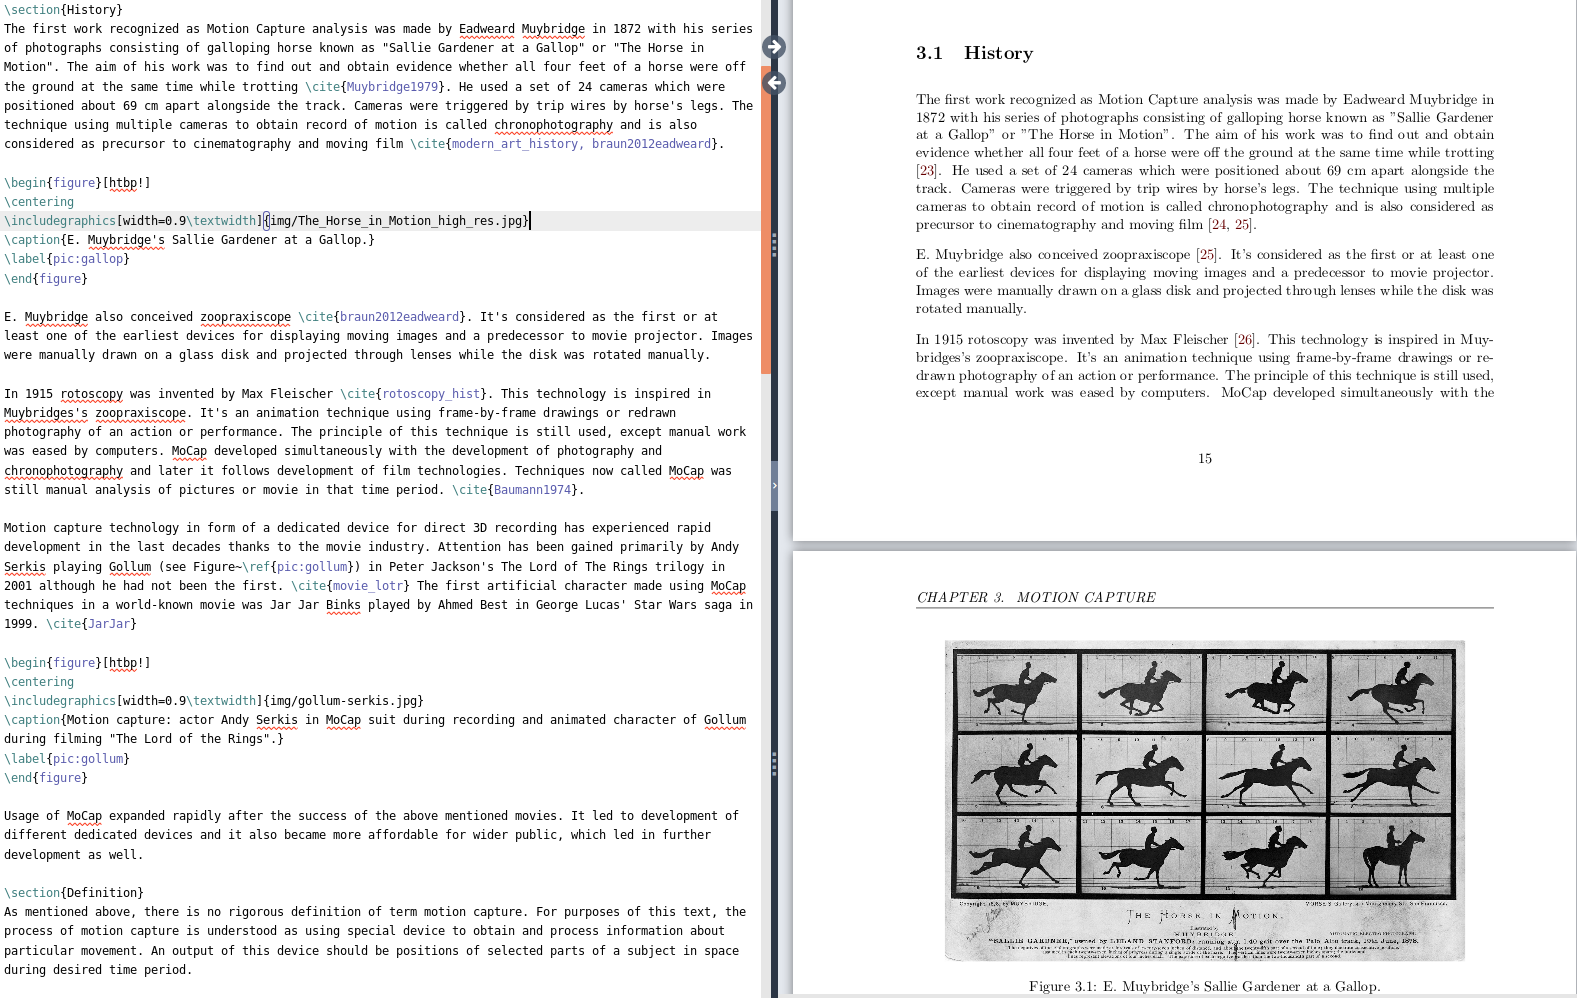
\includegraphics[width=\textwidth]{latex.png}
\end{frame}

\begin{frame}{Jak se v tom píše?}
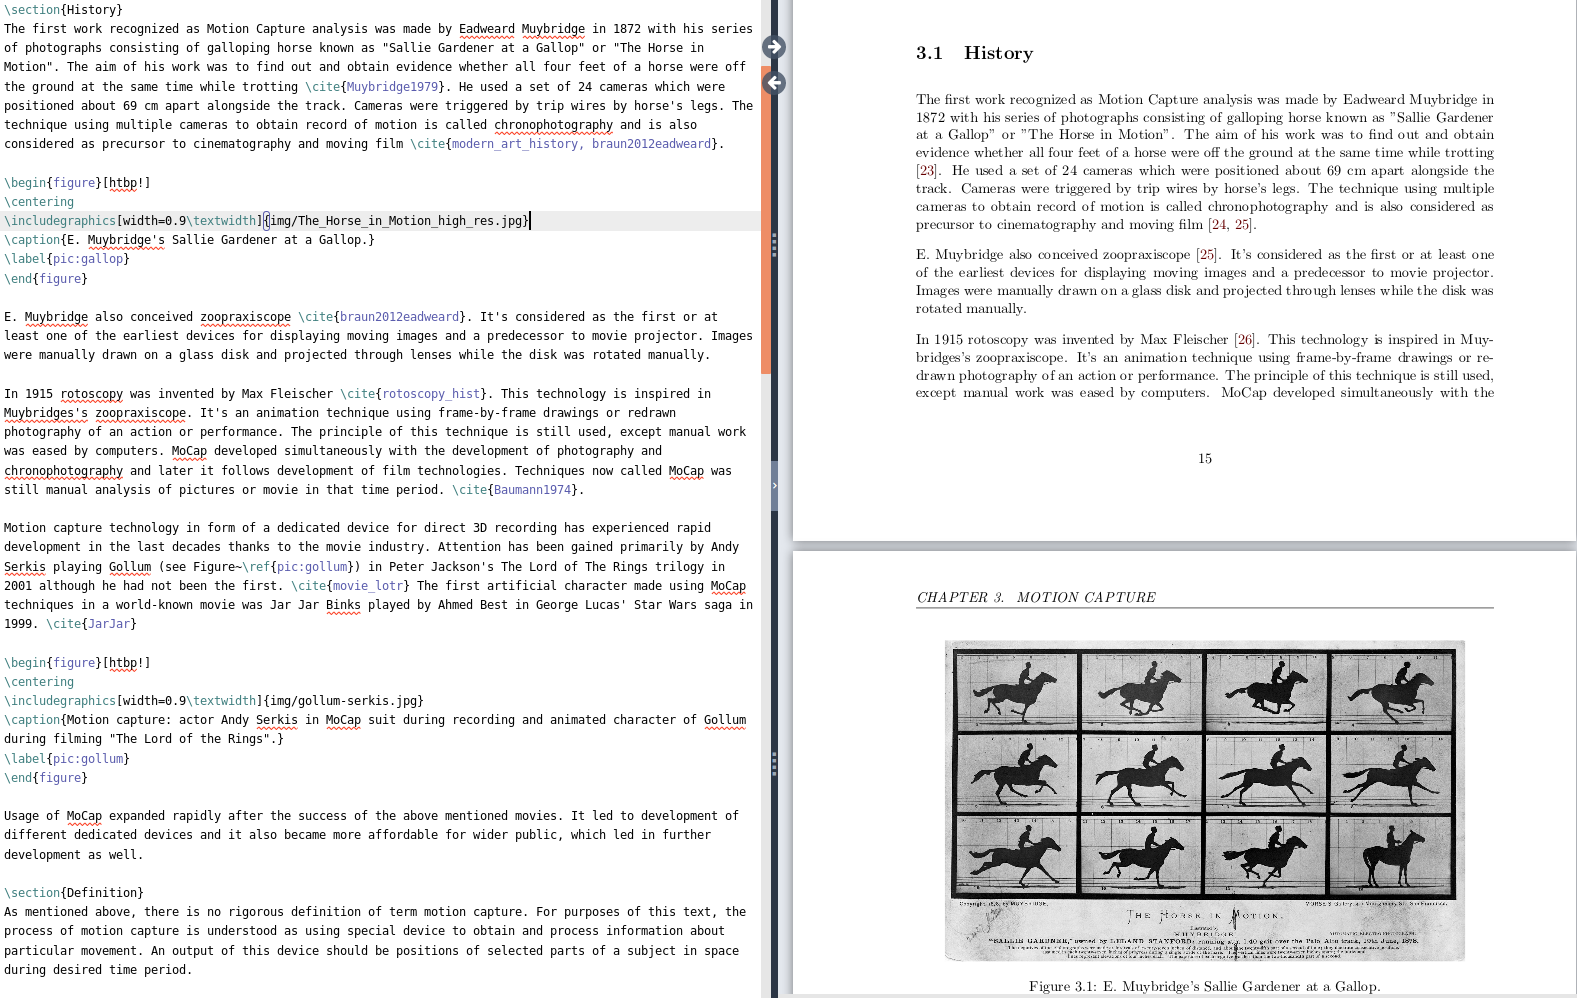
\includegraphics[width=2\textwidth]{latex.png}
\end{frame}
\section{teorie}
\begin{frame}{Jak se v tom píše?}
\begin{itemize}
    \item používání formátovacích příkazů (high descriptive markup)
    \item vzhled sazby se mění definicí stylu dokumentu 
    \item systém balíků pro doplňky
\end{itemize}
\end{frame}
\section{možnosti}
\begin{frame}[fragile]{A jak se v tom tedy píše?}
Několik \sout{základních} příkazů na ukázku:
\begin{itemize}
\item \begin{verbatim} \documentclass{} \end{verbatim}
\item \begin{verbatim} \usepackage{} \end{verbatim}
\item \begin{verbatim} \chapter{} \end{verbatim}
\item \begin{verbatim} \section{} \end{verbatim}
\item \begin{verbatim} \textbf{} \end{verbatim}
\item \begin{verbatim} \includegraphics[]{} \end{verbatim}
\item \begin{verbatim} \begin{_} ... \end{_} \end{verbatim}
\begin{itemize}
    \item document
    \item figure
\end{itemize}
\end{itemize}
\end{frame}

\begin{frame}{Co to umí?}
\begin{itemize}
    \item[]\textbf{rovnice:}
    
    \begin{align}
    E = mc^2 \\
    \forall \varepsilon > 0: \exists n \in \mathbb{N} : \forall k \geq n : \left| a _k - A \right| < \varepsilon \\
    f(x_1,x_2,...,x_s) = \frac{1}{\sqrt{{(2\pi)}^s {\left|\mathbf{C}\right|}}} \mathrm{e}^{-\frac{1}{2}{\left(\mathbf{x}-\mathbf{\mu}\right)}^T \mathbf{C}^{-1} {\left(\mathbf{x}-\mathbf{\mu}\right)}} \\
    F(x) = \int_{-\infty}^x \frac{1}{\sigma\sqrt{2\pi}} \mathrm{e}^{-\frac{{(t-\mu)}^2}{2\sigma^2}} \;\mathrm{d}t
    \end{align}

    \item[]\textbf{jiné písmo:}
    
\foreignlanguage{russian}{Союз нерушимый республик свободных \\
Сплотила навеки Великая Русь. \\
Да здравствует созданный волей народов \\
Единый, могучий Советский Союз!}
\end{itemize}
\end{frame}

\begin{frame}{Co to umí?}

 \begin{table}[h!]
\centering
\begin{tabular}{||c c c c||} 
 \hline
 Col1 & Col2 & Col2 & Col3 \\ [0.5ex] 
 \hline\hline
 1 & 6 & 87837 & 787 \\ 
 2 & 7 & 78 & 5415 \\
 3 & 545 & 778 & 7507 \\
 4 & 545 & 18744 & 7560 \\
 5 & 88 & 788 & 6344 \\ [1ex] 
 \hline
\end{tabular}
\caption{Table to test captions and labels}
\label{table:1}
\end{table}


\end{frame}

\begin{frame}{Co ještě to umí?}
\begin{figure}
    \centering
\begin{tikzpicture}[scale=0.8]
\begin{scope}[every node/.style={circle,thick,draw}]
    \node (A) at (0,0) {A};
    \node (B) at (0,3) {B};
    \node (C) at (2.5,4) {C};
    \node (D) at (2.5,1) {D};
    \node (E) at (2.5,-3) {E};
    \node (F) at (5,3) {F} ;
\end{scope}

\begin{scope}[>={Stealth[black]},
              every node/.style={fill=white,circle},
              every edge/.style={draw=red,very thick}]
    \path [->] (A) edge node {$5$} (B);
    \path [->] (B) edge node {$3$} (C);
    \path [->] (A) edge node {$4$} (D);
    \path [->] (D) edge node {$3$} (C);
    \path [->] (A) edge node {$3$} (E);
    \path [->] (D) edge node {$3$} (E);
    \path [->] (D) edge node {$3$} (F);
    \path [->] (C) edge node {$5$} (F);
    \path [->] (E) edge node {$8$} (F); 
    \path [->] (B) edge[bend right=60] node {$1$} (E); 
\end{scope}
\end{tikzpicture}
    
    \caption{Orientovaný graf.\footnote{Zdroj: TeX exchange, author: Torbjørn T.}}
    \label{fig:my_label}
\end{figure}



\end{frame}

\begin{frame}{Co ještě to umí?}
    \newgame
    \styleA
    %\hidemoves{1.g4 e5 2.f3 Qh4}
    \mainline{1.g4 e5; 2.f3 Qh4\footnote{Grob's attack f-pawn defence fail. }}
    \chessboard
\end{frame}

\begin{frame}{Už jste zahlceni informacemi?}
\begin{center}

\includegraphics[width=.8\textwidth]{pic/glum1.jpeg}
\footnote{Zdroj: Peter Jackson's The Lord of The Rings - Gollum}
\end{center}
\end{frame}
\begin{frame}{Zkusme udělat nějaký 'Hello world' dokument...}
\begin{center}
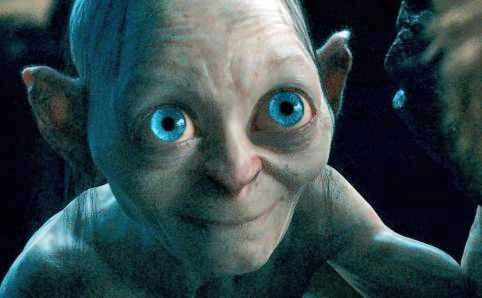
\includegraphics[width=.8\textwidth]{pic/glum2.jpg}
\footnote{Zdroj: Peter Jackson's The Lord of The Rings - Gollum}
\end{center}\end{frame}

\section{programy}
\begin{frame}{Kde si to můžu vyzkoušet?}
\begin{itemize}
    \item nainstalovat program (TexMaker, TeX studio, Lyx, TeXpen, Gummi, ..)
    \item online služba (Overleaf, Latexbase, ...)
\end{itemize}
\end{frame}
\section{overleaf}
\begin{frame}{Overleaf}
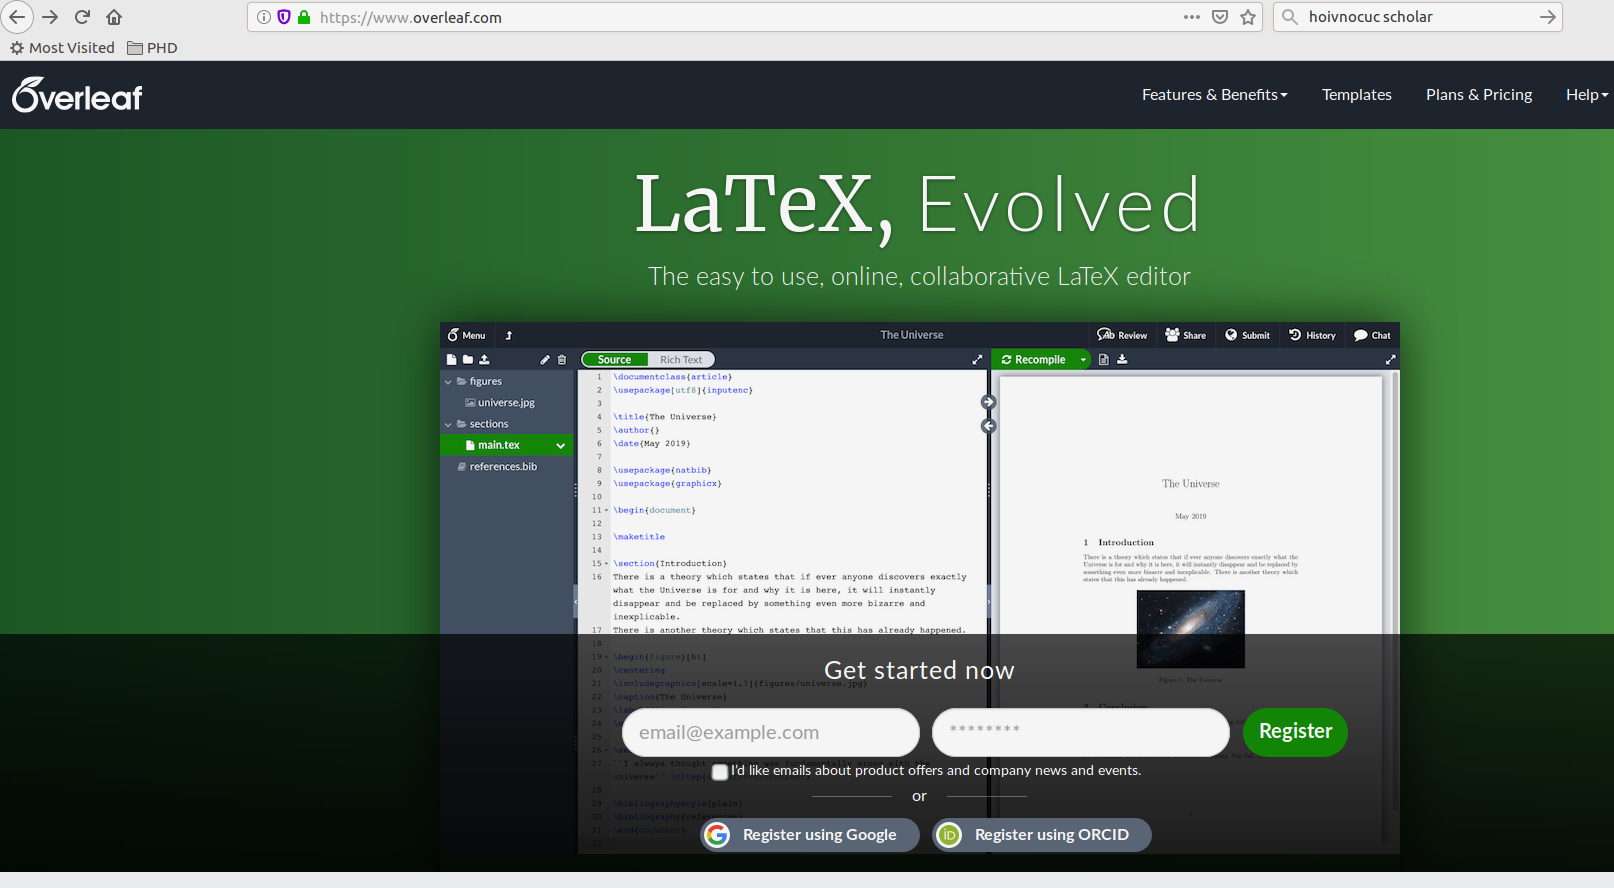
\includegraphics[width=\textwidth]{pic/over1.png}
\end{frame}
\begin{frame}{Overleaf}
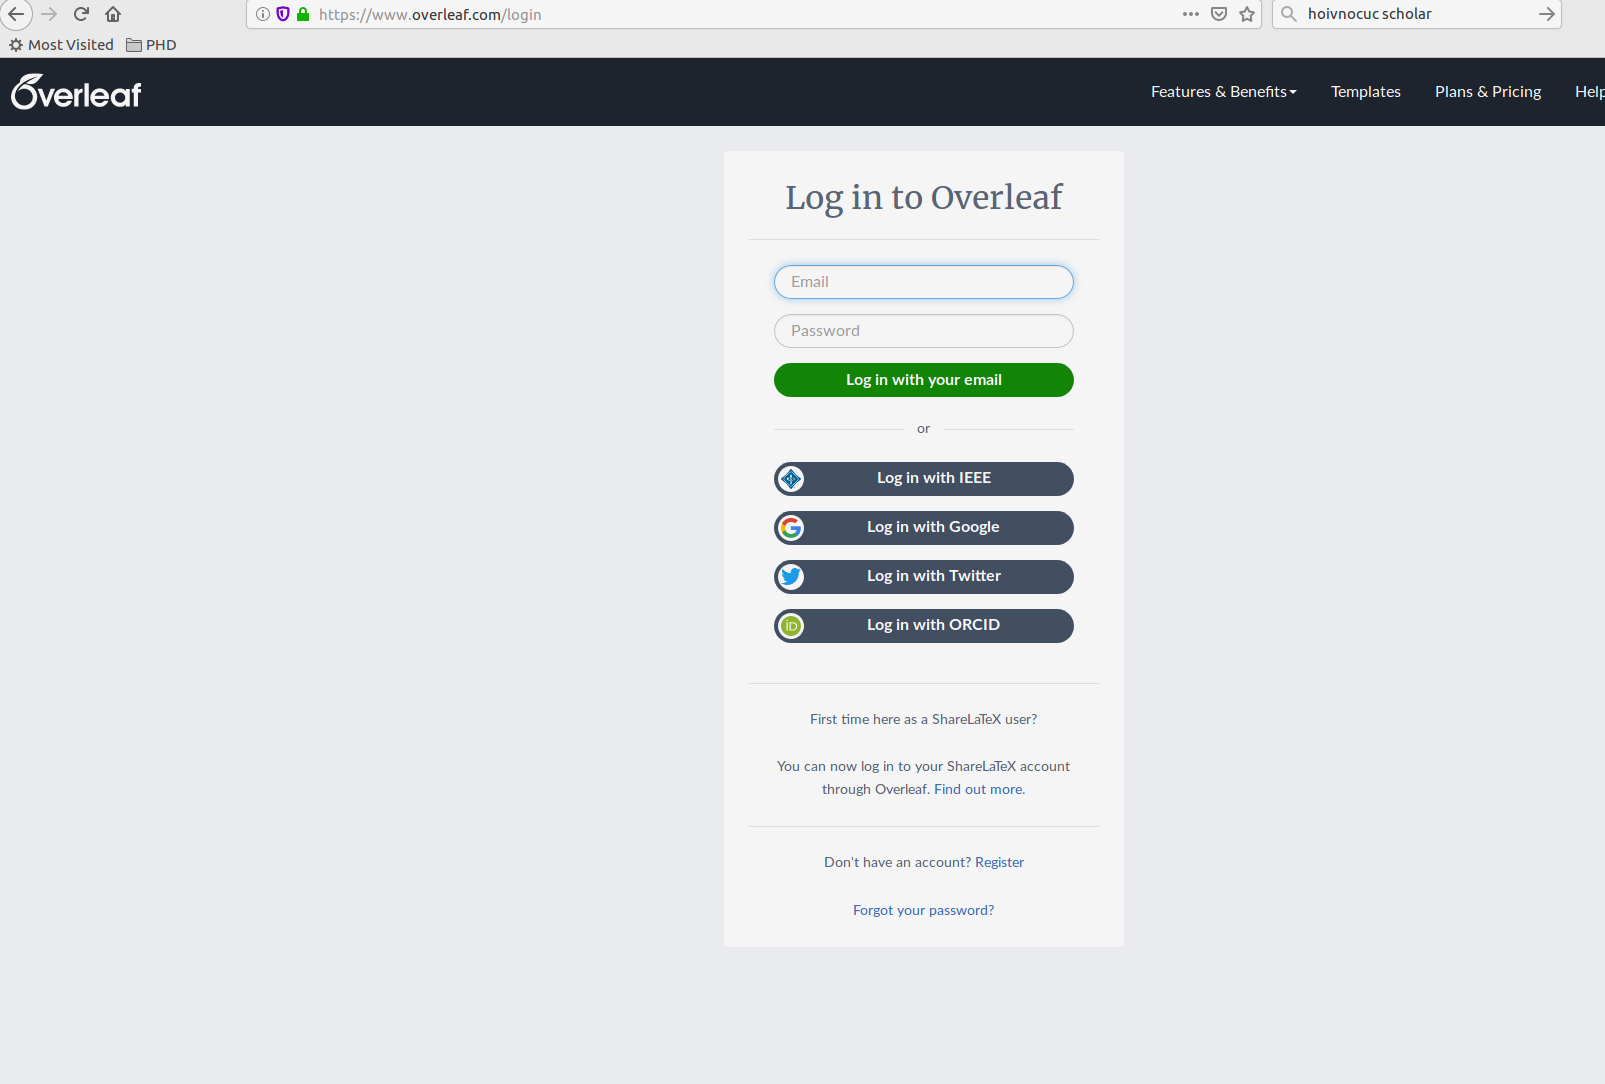
\includegraphics[width=\textwidth]{pic/over2.png}
\end{frame}
%\begin{frame}{Overleaf}
%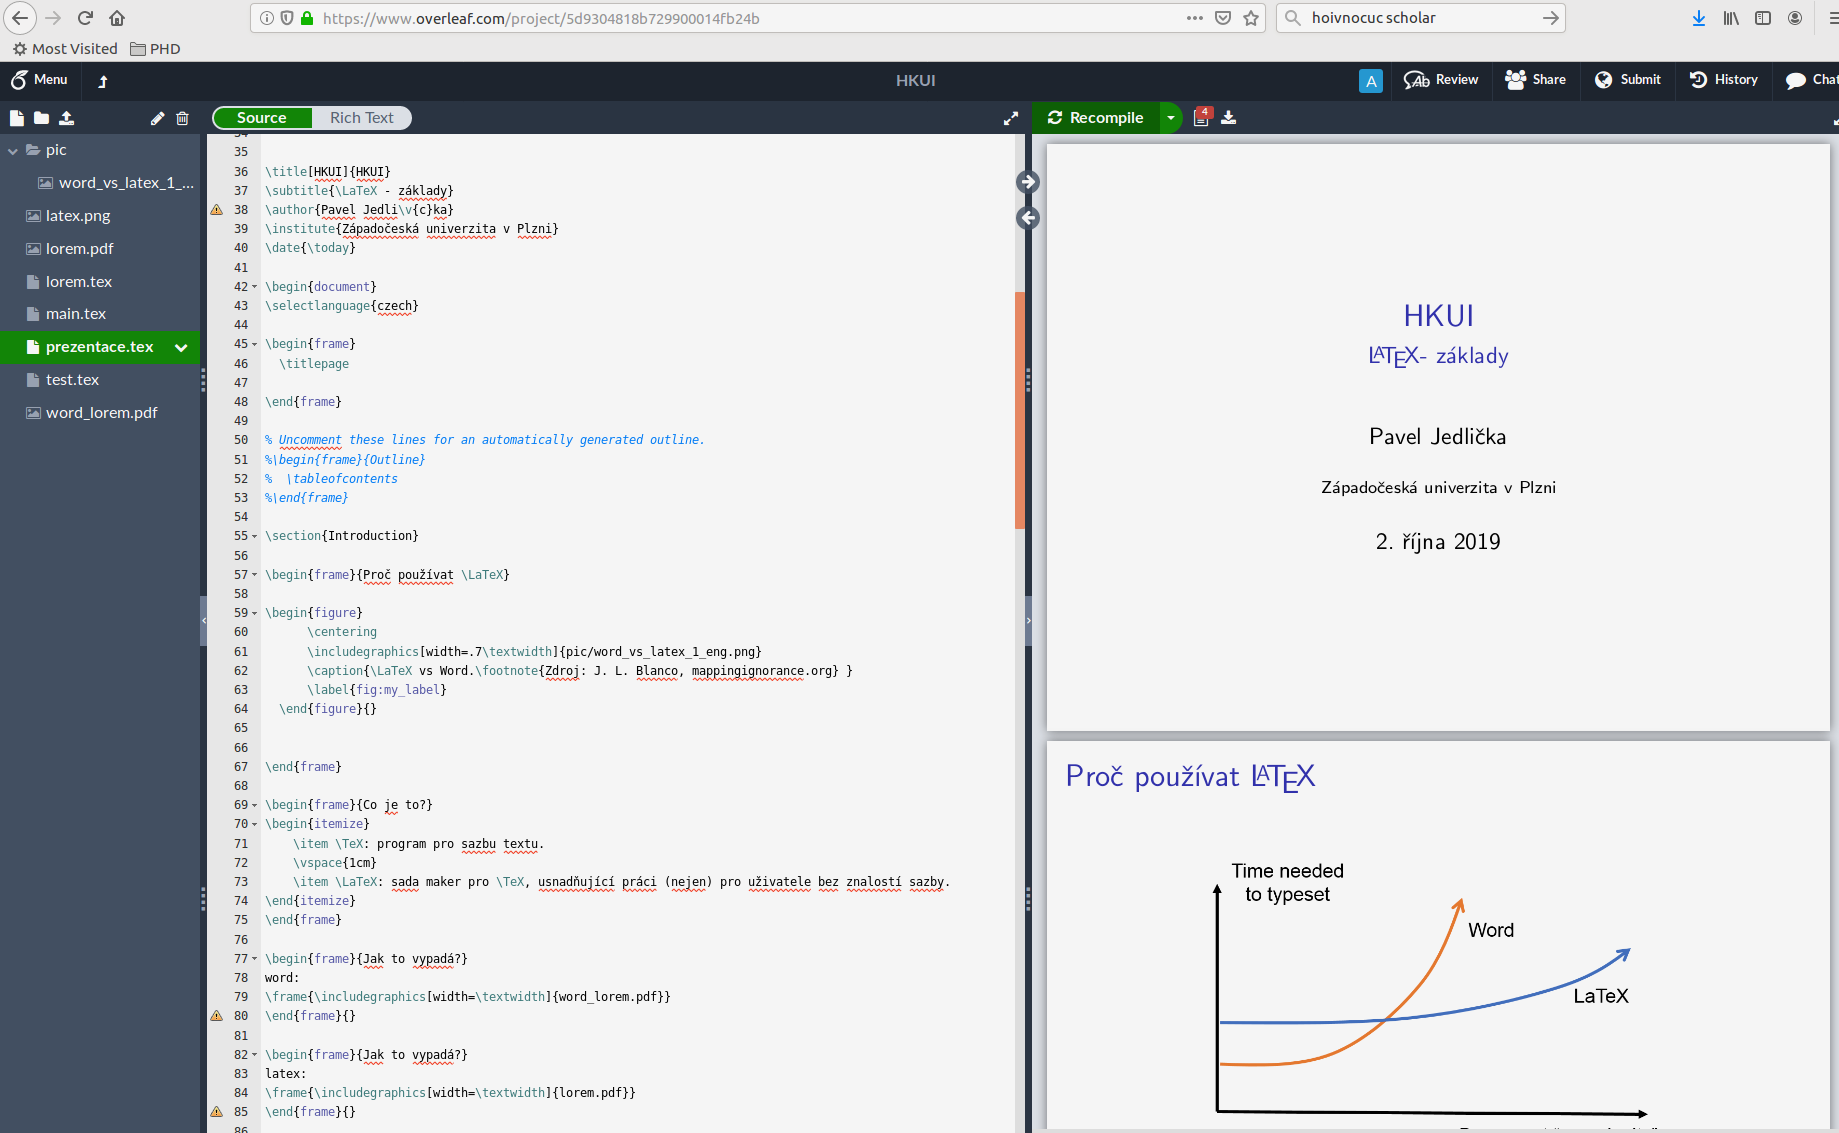
\includegraphics[width=\textwidth]{pic/over3.png}
%\end{frame}
\begin{frame}{Overleaf}
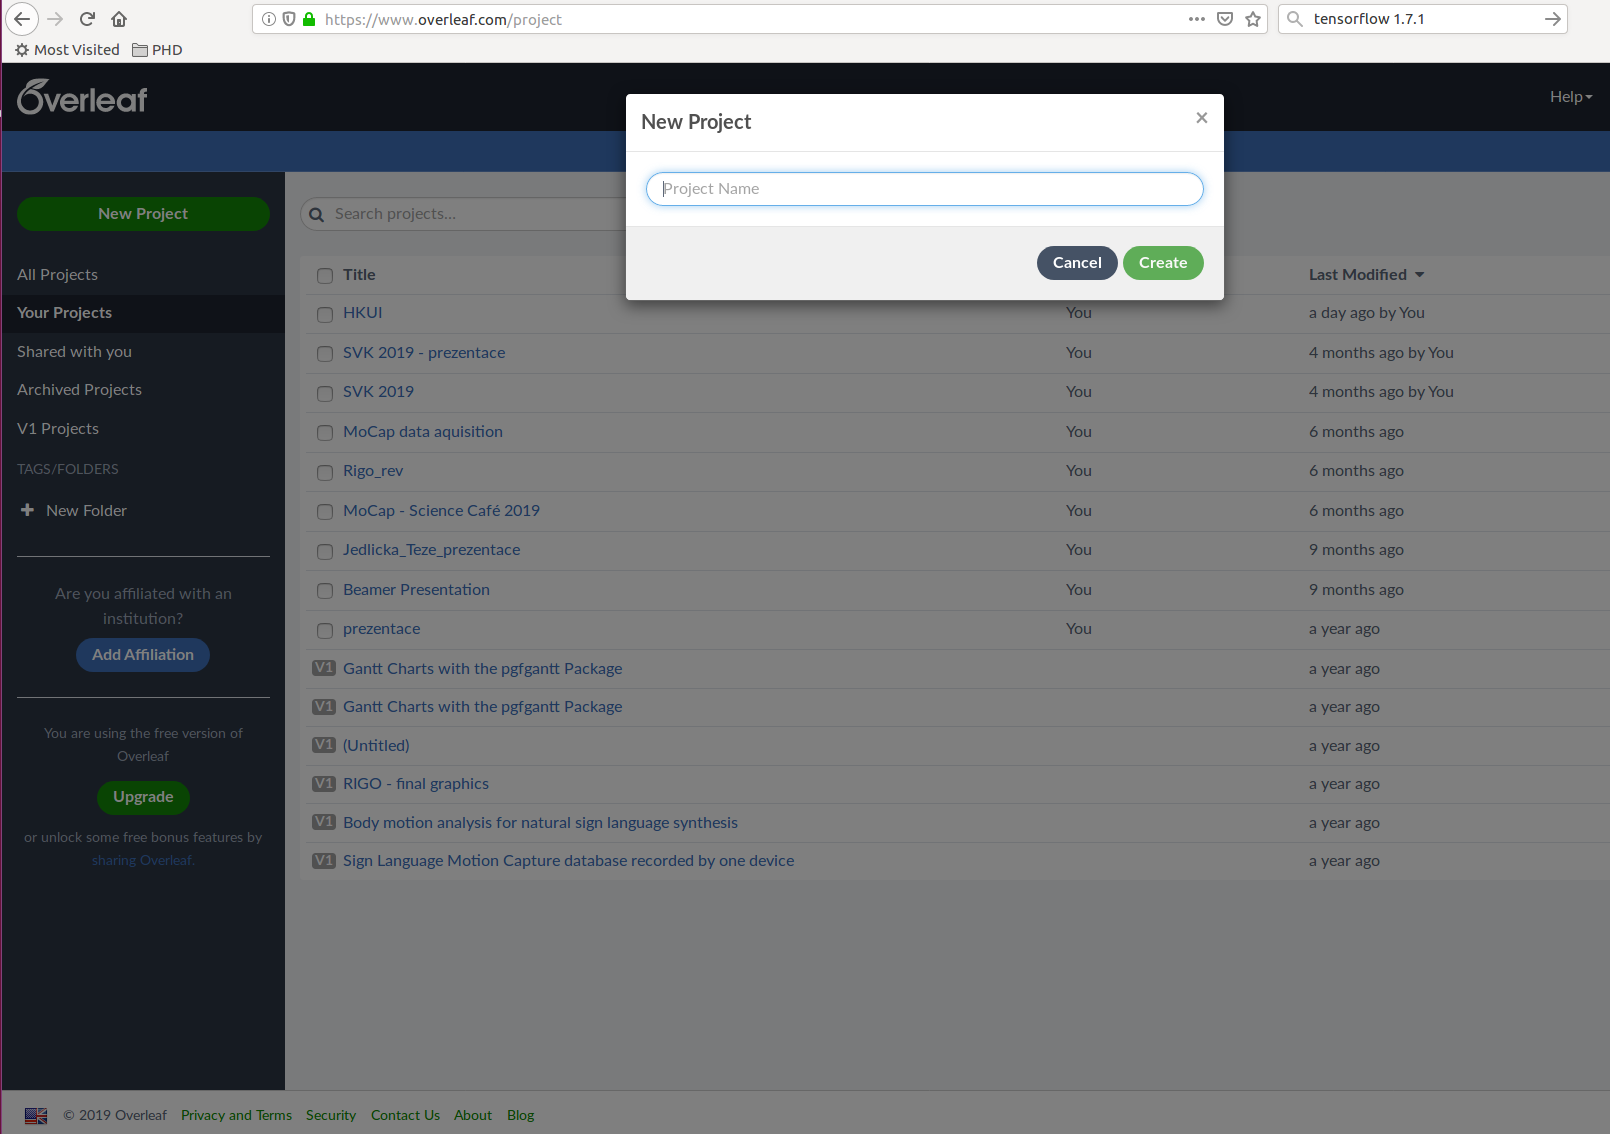
\includegraphics[width=\textwidth]{pic/over3p5.png}
\end{frame}
\begin{frame}{Overleaf}
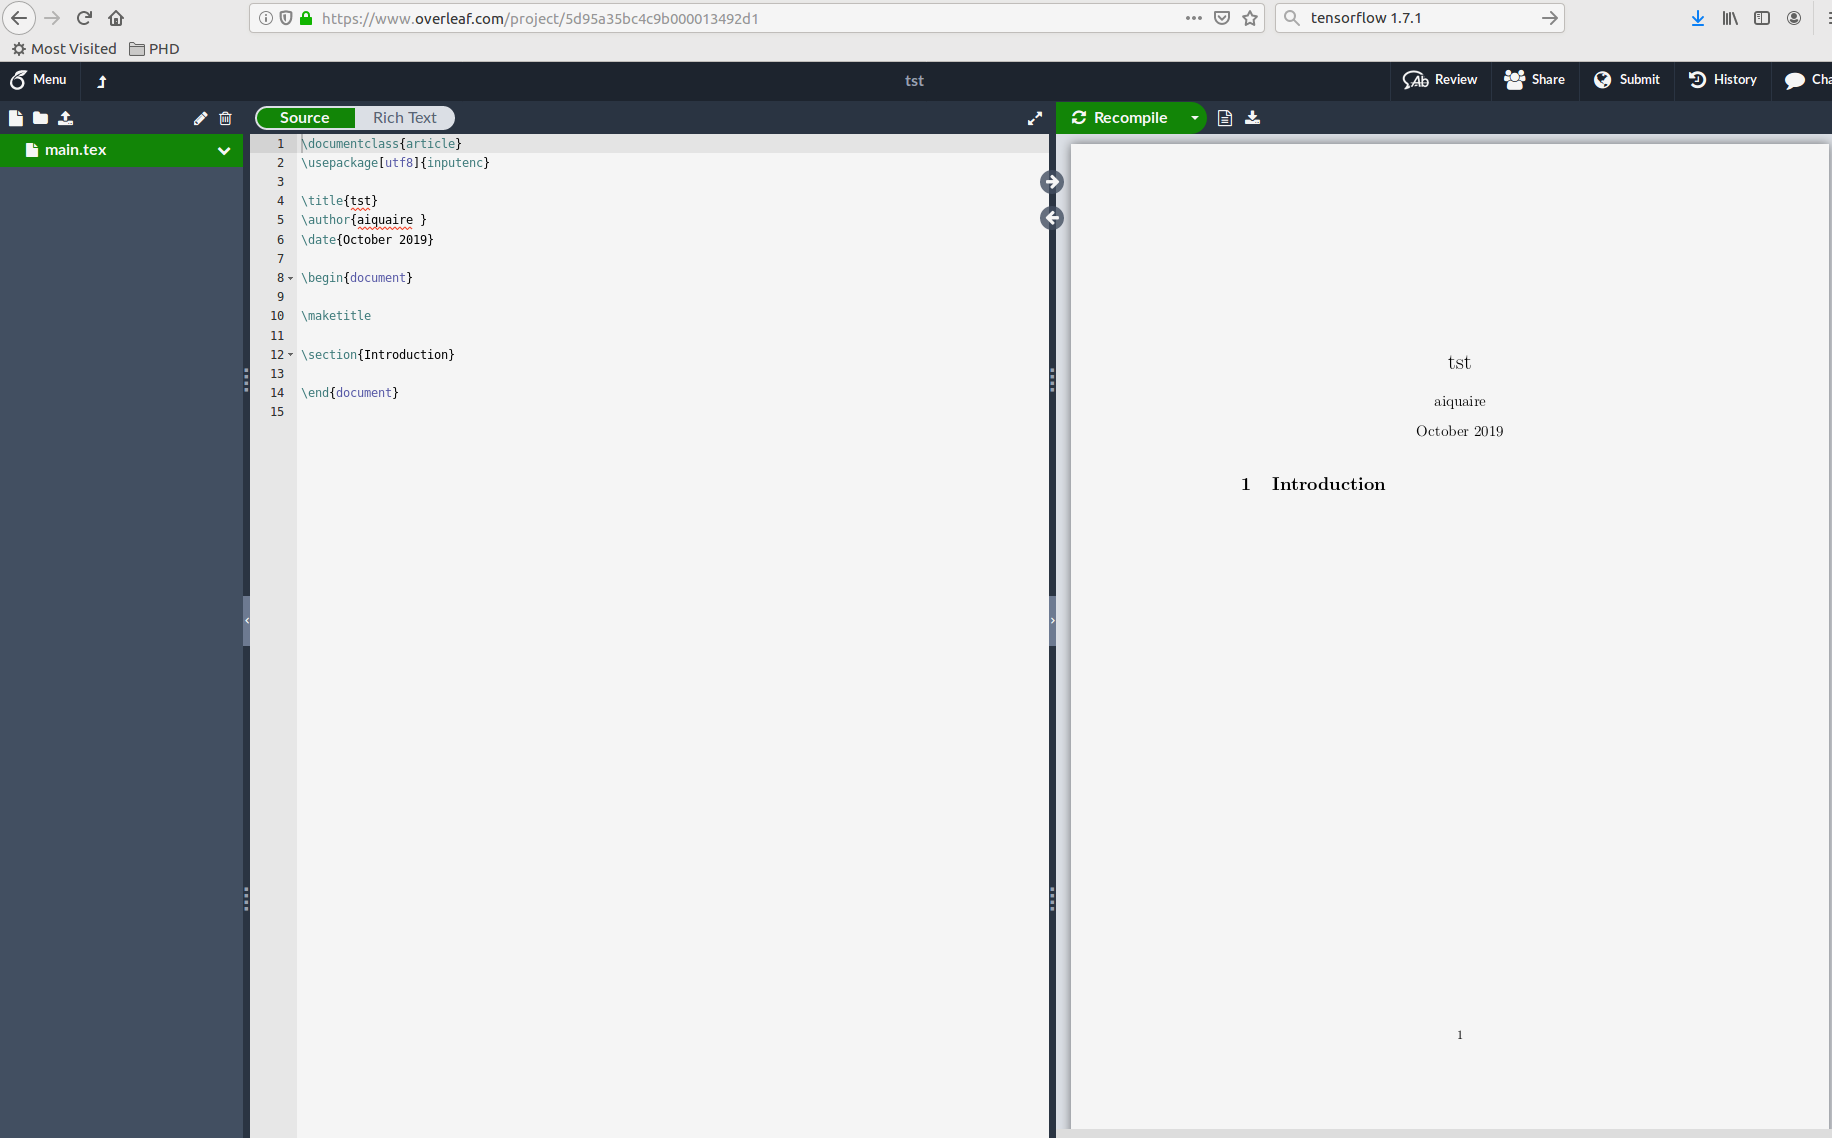
\includegraphics[width=\textwidth]{pic/over4.png}
\end{frame}
\begin{frame}{Overleaf}
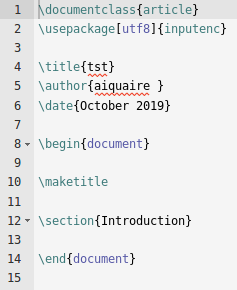
\includegraphics[width=0.7\textwidth]{pic/over5.png}
\end{frame}
\begin{frame}{Základní příkazy - documentclass}
\begin{itemize}
    \item \textbf{article} for articles in scientific journals, presentations, short reports, program documentation, invitations, ...
    \item \textbf{proc} a class for proceedings based on the article class.
    \item \textbf{minimal} is as small as it can get. It only sets a page size and a base font. It is mainly used for debugging purposes.
    \item \textbf{report} for longer reports containing several chapters, small books, thesis, ...
    \item \textbf{book} for real books
    \item \textbf{slides} for slides. The class uses big sans serif letters.
    \item \textbf{memoir} for changing sensibly the output of the document. It is based on the book class, but you can create any kind of document with it (1)
    \item \textbf{letter} For writing letters.
    \item \textbf{beamer} For writing presentations
\end{itemize}
\end{frame}

\begin{frame}{Zákldní informace - struktura dokumentu}
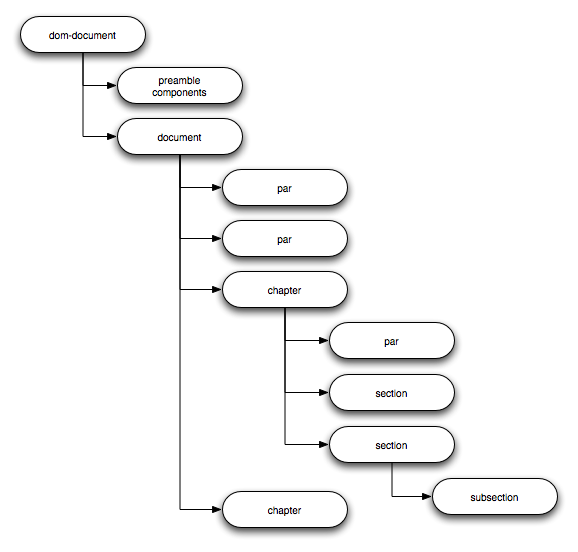
\includegraphics[width=.7\textwidth]{pic/docstruct.png}
\footnote{Zdroj: plasTeX - A Python Framework for Processing LaTeX Documents}
\end{frame}{}
\begin{frame}{Základní příkazy - usepackage}
    The Com­pre­hen­sive TeX Archive Net­work (CTAN) is the cen­tral place for all kinds of ma­te­rial around TeX and LaTeX. CTAN has cur­rently over \textbf{4,000 pack­ages}. Most of the pack­ages are free and can be down­loaded and used im­me­di­ately. \\
    \vspace{1cm}
    You can browse list of TeX and LaTeX packages and class files on CTAN subpage http://www.ctan.org/pkg/. 
\end{frame}


\begin{frame}{Bibtex}

Nástroj pro práci s literaturou

\begin{verbatim}
    This document is an example of BibTeX using in bibliography management. Three items 
are cited: \textit{The \LaTeX\ Companion} book \cite{latexcompanion}, the Einstein
journal paper \cite{einstein}, and the Donald Knuth's website \cite{knuthwebsite}. 
The \LaTeX\ related items are \cite{latexcompanion,knuthwebsite}. 

\medskip

\bibliographystyle{unsrt}
\bibliography{sample}
\end{verbatim}

Užitečné zejména s ve spojení s Mendeley nebo JabRef
    
\end{frame}




\begin{frame}{Děkuji za pozornost.}
\centering

\includegraphics[width=.8\textwidth]{pic/Thumbs-up.jpg}
\footnote{Obrázek: Interplay: Fallout}
\end{frame}





\end{document}
